\scanpage{85}
\mspage{10}
Un cas trivial intéressant est celui où $f$ est un isomorphisme --- et $=$ celui où $X=Y$, et où $f$ fait partie d'un groupe \inserted{$\mathcal G$} de $K$-isomorphismes de $X$ --- alors on peut considérer $\Pi_1(X)$ et $\Pi_1(X_{\bar K}),\Pi_1(X_K)$ comme des groupoïdes où opère $\mathcal G$, et $\widehat\Pi_1(X)$ comme un groupoïde où opère $\mathcal G\times\mathbf{\Gamma}$, $\widehat\Pi_1(\bar X_{\bar K})$ comme un groupoïde sur lequel $\mathcal G\times\Gamma$ opère. Cette fois-ci le groupe n'opère pas trivialement sur les sommets de $\Pi_1(X_K)$, l'opération de $\Gamma$ est triviale, mais pas nécessairement celle de $\mathcal G$.

Si on se donne un pt $x_0\in X_K$ comme pt base, et un ens de sommets $I\subset X_K$ contenant $x_0$, l'opération de $\Gamma$ sur $\widehat\Pi_1(X,I)$ est connue quand on \unsure{connait|connaît} son opération sur $\widehat\Pi_1(X,x_0)$, et si de plus on \unsure{connait|connaît} son opération sur les $\widehat\Pi_1(X,x_0)$-torseurs ! droit
\figure{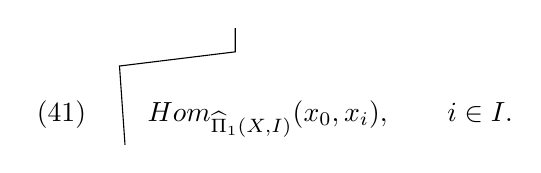
\begin{tikzpicture}
\node[anchor=base east] at(-.65,0) {$(41)$};
\node[anchor=base west,inner sep=0pt] at(0,0) {$\uline{\operatorname{Hom}}_{\widehat\Pi_1(X,I)}(x_0,x_i),\qquad i\in I.$};
\draw(-.28,-.30)--(-.35,.70)--(1.12,.88)--(1.12,1.18);
\end{tikzpicture}}
ou, ce qui revient au $=$, si on connait les
\margin{84}
